\chapter{विभव--pH आरेख}\label{ch:b1:e-ph-diagrams}

वर्षा के पानी में छोड़ी गई लोहे की कील में जंग लग जाती है; वही कील प्रबल
क्षारकीय विलयन में हफ़्तों तक चमकती रहती है। किसी जहाज़ के इस्पात के ढाँचे पर
ज़िंक के ब्लॉक लगे होते हैं जो उसके स्थान पर घुलते हैं, और ताँबे की छत हरी
पड़ जाती है पर कभी लुप्त नहीं होती। pH पर निर्भर विभव वाले \omterm{def:b1:nernst:couple}{अपचयोपचय युग्म},
हाइड्रॉक्साइडों और ऑक्साइडों का अवक्षेपण, अम्ल--क्षारक साम्य: तीनों
एक साथ काम करते हैं, और एक ही मानचित्र उन्हें इकट्ठा करता है। pH के सापेक्ष
विभव के आलेख पर किसी तत्व की हर स्पीशीज़ को वह क्षेत्र मिलता है जहाँ वह
स्थायी रूप है; मानचित्र पढ़कर पता चलता है कि पानी में कौन-सी स्पीशीज़ टिकती हैं, कौन-सी
आपस में अभिक्रिया करती हैं, और कोई धातु कहाँ संक्षारित होती है।

\begin{recall}
\omterm{thm:b1:nernst:nernst}{नेर्न्स्ट समीकरण}, \omterm{def:b1:nernst:electrode-potential}{मानक विभव} और अपचयोपचय अभिक्रियाओं का पूर्वानुमान
\cref{ch:b1:nernst} में हैं; \omterm{def:b1:predominant-reaction:predominance}{प्रभाविता आरेख}
\cref{ch:b1:predominant-reaction} में; हाइड्रॉक्साइडों की अवक्षेपण-सीमाएँ और
ठोसों के \omterm{def:b1:precipitation:existence-domain}{अस्तित्व क्षेत्र} \cref{ch:b1:precipitation} में।
सभी विभव \qty{25}{\celsius} पर हैं, $RT\ln 10/F = \qty{0.059}{V}$ के साथ।
\end{recall}

\begin{omfigure}
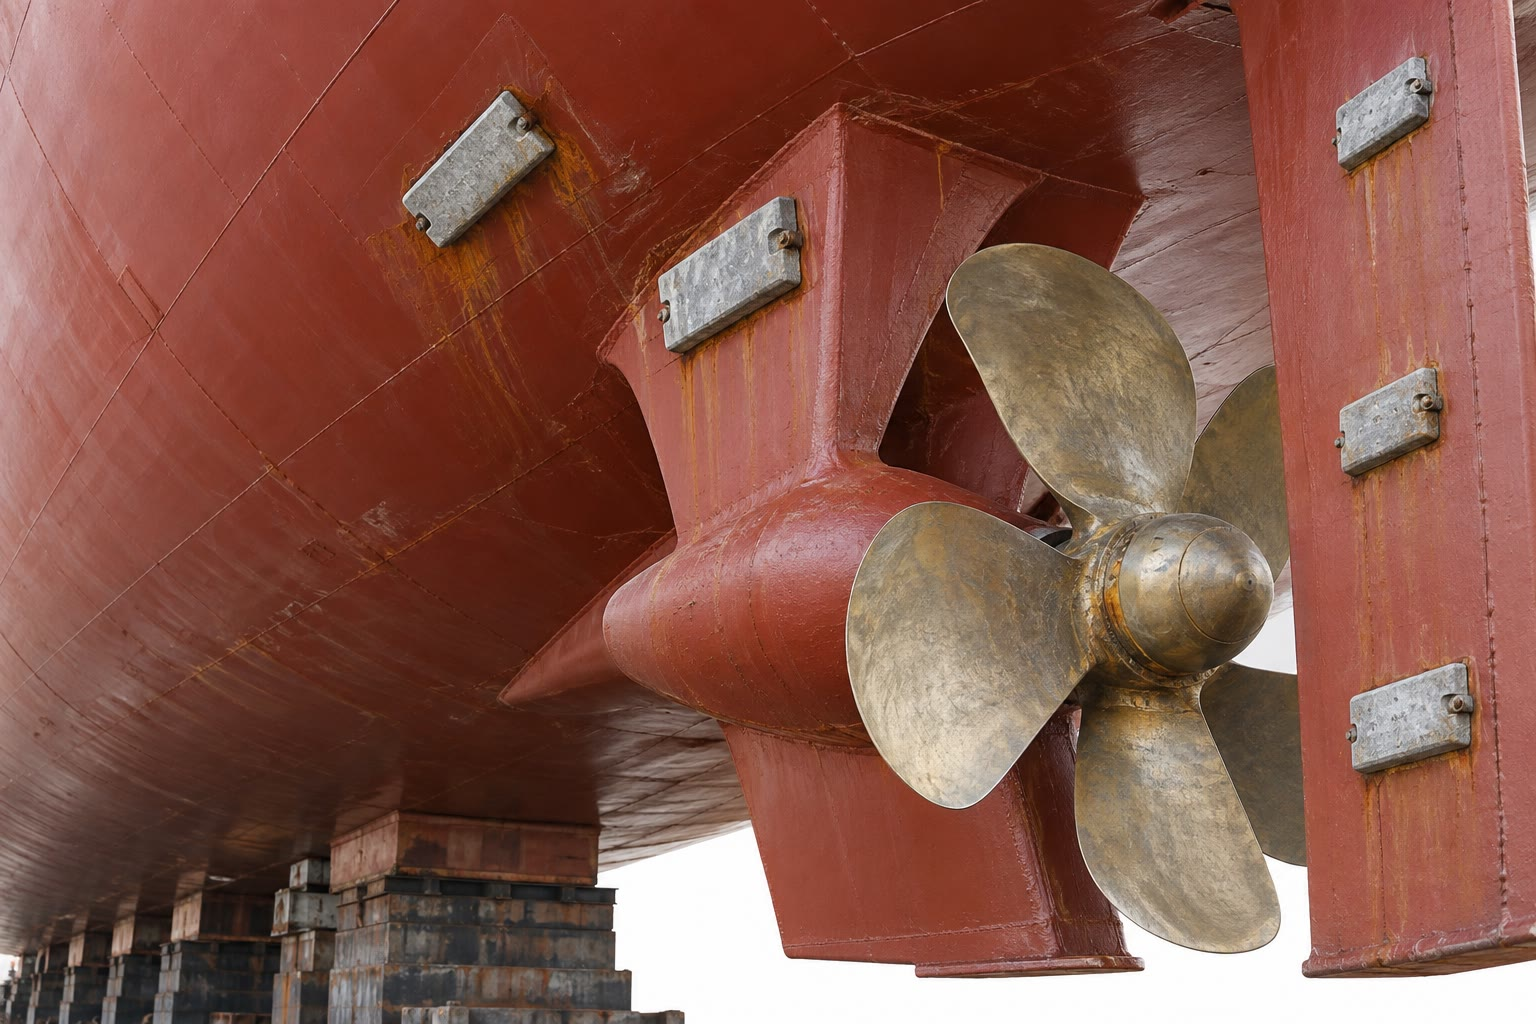
\includegraphics[width=0.6\linewidth]{images/book2/ai/b1-14-ship-anodes.jpg}

{\small सूखी गोदी में किसी जहाज़ का पिछला भाग। प्रोपेलर के पास ढाँचे पर लगे
धूसर ब्लॉक ज़िंक के हैं: समुद्री पानी में वे इस्पात के बजाय
संक्षारित होते हैं (\cref{exo:b1:e-ph-diagrams:12})।}
\end{omfigure}

\section{परिपाटियाँ}

\begin{definition}[विभव--pH आरेख, कार्यकारी सांद्रता]\label{def:b1:e-ph-diagrams:e-ph-diagram}
किसी तत्व का \emph{विभव--pH आरेख}\index{विभव--pH आरेख}
क्षेत्रों में बँटा तल $(\mathrm{pH}, E)$ है, जिसमें हर क्षेत्र तत्व के किसी एक रूप का
प्रभाविता क्षेत्र (घुली स्पीशीज़) या \omterm{def:b1:precipitation:existence-domain}{अस्तित्व क्षेत्र} (ठोस) है। इसे एक चुनी हुई
\emph{कार्यकारी सांद्रता}\index{कार्यकारी सांद्रता} $c$ के लिए बनाया जाता है, जो
विलयन में तत्व की कुल सांद्रता है, इन परिपाटियों के साथ:
\begin{itemize}
  \item दो घुली स्पीशीज़ के बीच की सीमा पर हर एक $c$ पर होती है
        (तत्व के परमाणुओं में गिनकर);
  \item किसी घुली स्पीशीज़ और किसी ठोस के बीच की सीमा पर
        घुली स्पीशीज़ $c$ पर होती है और ठोस बस उपस्थित होता है;
  \item गैसें \qty{1}{bar} पर होती हैं।
\end{itemize}
इस अध्याय में $c = \qty{0.010}{mol/L}$।
\end{definition}

तत्व के रूपों को \omterm{def:b1:nernst:oxidation-number}{ऑक्सीकरण संख्या} के क्रम में रखा जाता है: संख्या जितनी ऊँची,
आरेख पर उतना ऊपर (ऑक्सीकृत रूप ऊँचे विभव पर स्थायी होते हैं)।
किसी दी गई \omterm{def:b1:nernst:oxidation-number}{ऑक्सीकरण संख्या} पर अधिक क्षारकीय रूप
(हाइड्रॉक्साइड, ऑक्साइड, हाइड्रॉक्सो \omterm{def:b1:complexation:complex}{संकुल}) दाईं ओर होते हैं।

\begin{proposition}[सीमा की प्रवणता]\label{prop:b1:e-ph-diagrams:boundary-slope}
भिन्न \omterm{def:b1:nernst:oxidation-number}{ऑक्सीकरण संख्याओं} वाली दो स्पीशीज़ के बीच की सीमा, जिसका
\omterm{def:b1:nernst:couple}{अर्ध-समीकरण} $n$ इलेक्ट्रॉनों और $m$ प्रोटॉनों का विनिमय करता है,
$\mathrm{Ox} + m\,\ce{H+} + n\,\mathrm{e^-} \rightleftharpoons \mathrm{Red} +
\cdots$, प्रति pH इकाई $-0.059\,m/n$ वोल्ट प्रवणता वाली सरल रेखा है। समान
\omterm{def:b1:nernst:oxidation-number}{ऑक्सीकरण संख्या} वाली दो स्पीशीज़ के बीच की सीमा ऊर्ध्वाधर होती है।
\end{proposition}

\begin{proof}
\omterm{thm:b1:nernst:nernst}{नेर्न्स्ट समीकरण} देता है $E = E^\circ + \frac{0.059}{n}\log\frac{[\mathrm{Ox}]
[\ce{H+}]^m}{[\mathrm{Red}]} = E^\circ + \frac{0.059}{n}\log\frac{[\mathrm{Ox}]}
{[\mathrm{Red}]} - \frac{0.059\,m}{n}\,\mathrm{pH}$, और सीमा पर
सांद्रताएँ परिपाटियों से तय होती हैं। समान
\omterm{def:b1:nernst:oxidation-number}{ऑक्सीकरण संख्या} वाली दो स्पीशीज़ इलेक्ट्रॉन-रहित किसी अम्ल--क्षारक या अवक्षेपण साम्य से
जुड़ी होती हैं, जिसका स्थिरांक सीमा का pH तय करता है,
विभव चाहे जो हो।
\end{proof}

\section{पानी}

\begin{proposition}[पानी की दो रेखाएँ]\label{prop:b1:e-ph-diagrams:water-lines}
गैस के \qty{1}{bar} के अंतर्गत पानी रेखा
$E = -0.059\,\mathrm{pH}$ के नीचे हाइड्रोजन में अपचित होता है और रेखा $E = 1.23
- 0.059\,\mathrm{pH}$ के ऊपर ऑक्सीजन में ऑक्सीकृत।
\end{proposition}

\begin{proof}
\ce{2H+ + 2e- -> H2}: $E = 0 + \frac{0.059}{2}\log\frac{[\ce{H+}]^2}{p(\ce{H2})}
= -0.059\,\mathrm{pH}$, $p = 1$ पर। \ce{O2 + 4H+ + 4e- -> 2H2O}: $E = 1.23 +
\frac{0.059}{4}\log(p(\ce{O2})[\ce{H+}]^4) = 1.23 - 0.059\,\mathrm{pH}$। पहली
रेखा के नीचे \ce{H2} युग्म का स्थायी रूप है (पानी
अपचित होता है); दूसरी के ऊपर \ce{O2}।
\end{proof}

\begin{definition}[जल का स्थायित्व क्षेत्र]\label{def:b1:e-ph-diagrams:water-domain}
दोनों रेखाओं के बीच की पट्टी, जो हर pH पर \qty{1.23}{V} चौड़ी है,
\emph{जल का स्थायित्व क्षेत्र}\index{जल का स्थायित्व क्षेत्र} है: जिस
स्पीशीज़ का क्षेत्र पूरी तरह इसके भीतर हो, वह न पानी को ऑक्सीकृत करती है न
अपचित।
\end{definition}

\section{आरेख बनाना: आयरन}

\begin{method}[विभव--pH आरेख बनाना]\label{met:b1:e-ph-diagrams:build}
\begin{enumerate}
  \item स्पीशीज़ सूचीबद्ध कीजिए और उन्हें \omterm{def:b1:nernst:oxidation-number}{ऑक्सीकरण संख्या} के क्रम में रखिए: आयरन के लिए
        \ce{Fe} (0), \ce{Fe^2+} और \ce{Fe(OH)2} ($+$II), \ce{Fe^3+} और
        \ce{Fe(OH)3} ($+$III)।
  \item हर \omterm{def:b1:nernst:oxidation-number}{ऑक्सीकरण संख्या} पर, \omterm{def:b1:e-ph-diagrams:e-ph-diagram}{कार्यकारी
        सांद्रता} पर अवक्षेपण (या अम्ल--क्षारक) साम्यों से ऊर्ध्वाधर सीमाएँ ज्ञात कीजिए
        (\cref{ch:b1:precipitation})।
  \item पड़ोसी \omterm{def:b1:nernst:oxidation-number}{ऑक्सीकरण संख्याओं} के हर जोड़े के लिए हर pH परास में
        \omterm{def:b1:nernst:couple}{अर्ध-समीकरण} और परिपाटियों के साथ उसका \omterm{thm:b1:nernst:nernst}{नेर्न्स्ट समीकरण} लिखिए;
        इससे ज्ञात प्रवणता वाली एक सरल सीमा मिलती है।
  \item रेखाओं को बाएँ से दाएँ जोड़िए; जहाँ तीन रेखाएँ मिलती हैं,
        वहाँ हर रेखा केवल उस ओर जारी रहती है जहाँ उसकी दोनों स्पीशीज़
        स्थायी हों।
  \item जाँचिए: क्षेत्र एक-दूसरे पर नहीं चढ़ने चाहिए, और प्रवणताएँ
        \cref{prop:b1:e-ph-diagrams:boundary-slope} से मेल खानी चाहिए।
\end{enumerate}
\end{method}

\begin{example}[आयरन की सीमाएँ]\label{ex:b1:e-ph-diagrams:iron}
$c = \qty{0.010}{mol/L}$ के साथ (और \cref{ch:b1:precipitation,ch:b1:nernst} के स्थिरांकों से):
\begin{itemize}
  \item \ce{Fe^3+}/\ce{Fe(OH)3}: $\mathrm{pH} = 14.00 - \frac13(38.55 - 2) = 1.82$;
        \ce{Fe^2+}/\ce{Fe(OH)2}: $\mathrm{pH} = 14.00 - \frac12(16.31 - 2) = 6.85$।
  \item \ce{Fe^2+}/\ce{Fe}: $E = -0.41 + 0.030\log c = -0.47$~V (pH 6.85 से नीचे)।
  \item \ce{Fe^3+}/\ce{Fe^2+}: $E = 0.77$~V (दोनों $c$ पर, pH 1.82 से नीचे)।
  \item \ce{Fe(OH)3}/\ce{Fe^2+}: \ce{Fe(OH)3 + 3H+ + e- -> Fe^2+ + 3H2O}, प्रवणता
        $-0.177$: pH 1.82 और 6.85 के बीच $E = 1.09 - 0.177\,\mathrm{pH}$।
  \item \ce{Fe(OH)3}/\ce{Fe(OH)2}: एक इलेक्ट्रॉन, एक प्रोटॉन, $E = 0.28 -
        0.059\,\mathrm{pH}$; \ce{Fe(OH)2}/\ce{Fe}: दो इलेक्ट्रॉन, दो
        प्रोटॉन, $E = -0.07 - 0.059\,\mathrm{pH}$ (pH 6.85 से ऊपर)।
\end{itemize}
अंतःखंड त्रिक बिंदुओं पर सातत्य से, या
सीधे विरचन की गिब्ज़ ऊर्जाओं से प्राप्त होते हैं; नीचे का आरेख
दूसरी विधि से परिकलित है, और इसकी सीमाएँ इन पूर्णांकित
मानों से \qty{0.01}{V} या 0.01 pH इकाई से कम भिन्न हैं।
% ledger: dfg:Fe2+_ao, dfg:Fe3+_ao, dfg:Fe_OH2_cr, dfg:Fe_OH3_cr, dfg:H2O_l, dfg:OH-_ao (boundaries computed in figdata/bachelor-1/eph-diagrams.py)
\end{example}

\begin{omfigure}
\begin{tikzpicture}
\begin{axis}[
  width=0.8\linewidth, height=8.2cm, xmin=0, xmax=14, ymin=-1.2, ymax=1.6,
  axis x line=bottom, axis y line=left, xlabel={pH}, ylabel={$E$ (V)},
  xtick={0,2,4,6,8,10,12,14}, ytick={-1,-0.5,0,0.5,1,1.5},
  unbounded coords=jump, clip=true,
  tick label style={font=\small}, label style={font=\small}]
\addplot[black!45, dashed] table[x=pH, y=H2] {figdata/out/bachelor-1-eph-diagrams-water.dat};
\addplot[black!45, dashed] table[x=pH, y=O2] {figdata/out/bachelor-1-eph-diagrams-water.dat};
\addplot[omDef, very thick] table[x=pH, y=E] {figdata/out/bachelor-1-eph-diagrams-iron.dat};
\node[font=\small] at (axis cs:3.2,-0.85) {\ce{Fe}};
\node[font=\small] at (axis cs:3.4,0.15) {\ce{Fe^2+}};
\node[font=\small] at (axis cs:0.9,1.45) {\ce{Fe^3+}};
\node[font=\small] at (axis cs:8.5,0.25) {\ce{Fe(OH)3}};
\node[font=\scriptsize] at (axis cs:11.0,-0.56) {\ce{Fe(OH)2}};
\node[font=\scriptsize, black!55, rotate=-14, anchor=south] at (axis cs:12.0,0.52) {\ce{O2}/\ce{H2O}};
\node[font=\scriptsize, black!55, rotate=-14, anchor=south] at (axis cs:2.2,-0.11) {\ce{H2O}/\ce{H2}};
\end{axis}
\end{tikzpicture}

{\small $c = \qty{0.010}{mol/L}$ के लिए आयरन का \omterm{def:b1:e-ph-diagrams:e-ph-diagram}{विभव--pH आरेख} (ठोस
रेखाएँ), पानी की दोनों रेखाओं (डैश) के साथ। हर सीमा
सारणीबद्ध विरचन गिब्ज़ ऊर्जाओं से परिकलित है।}
\end{omfigure}

\section{कॉपर और ज़िंक}

यही विधि कॉपर के आरेख (स्पीशीज़ \ce{Cu}, \ce{Cu+},
$+$I पर \ce{Cu2O}, \ce{Cu^2+}, $+$II पर \ce{CuO}) और ज़िंक के आरेख (\ce{Zn},
\ce{Zn^2+}, \ce{Zn(OH)2}, \ce{Zn(OH)4^2-}) भी देती है। कॉपर के लिए \ce{CuO}
$\mathrm{pH} = 14.00 - \frac12(20.64 - 2) = 4.68$ पर प्रकट होता है, और \ce{Cu+} आयन, सूची में होते हुए भी,
किसी क्षेत्र का स्वामी नहीं: अम्ल में $E^\circ(\ce{Cu+}/\ce{Cu}) = 0.52$~V,
$E^\circ(\ce{Cu^2+}/\ce{Cu+}) = 0.16$~V से ऊपर है, इसलिए उसका संभावित क्षेत्र
दोनों पड़ोसियों द्वारा काट दिया जाता है (\cref{sec:b1:e-ph-diagrams:reading})।
ज़िंक के लिए हाइड्रॉक्साइड pH 6.81 पर प्रकट होता है और इस सांद्रता पर
केवल 13.97 से ऊपर \ce{Zn(OH)4^2-} के रूप में फिर घुलता है, दाएँ किनारे पर
एक पतली पट्टी।

\begin{omfigure}
\begin{tikzpicture}
\begin{axis}[name=cu,
  width=0.47\linewidth, height=7cm, xmin=0, xmax=14, ymin=-1.4, ymax=1.6,
  axis x line=bottom, axis y line=left, xlabel={pH}, ylabel={$E$ (V)},
  xtick={0,4,8,12}, ytick={-1,-0.5,0,0.5,1,1.5},
  unbounded coords=jump, clip=true,
  tick label style={font=\small}, label style={font=\small}]
\addplot[black!45, dashed] table[x=pH, y=H2] {figdata/out/bachelor-1-eph-diagrams-water.dat};
\addplot[black!45, dashed] table[x=pH, y=O2] {figdata/out/bachelor-1-eph-diagrams-water.dat};
\addplot[omDef, very thick] table[x=pH, y=E] {figdata/out/bachelor-1-eph-diagrams-copper.dat};
\node[font=\small] at (axis cs:5,-0.7) {\ce{Cu}};
\node[font=\small] at (axis cs:2,0.7) {\ce{Cu^2+}};
\node[font=\small] at (axis cs:9.5,0.75) {\ce{CuO}};
\node[font=\scriptsize] (cuo) at (axis cs:11.8,-1.05) {\ce{Cu2O}};
\draw[->, black!70] (cuo.north) -- (axis cs:10,-0.035);
\node[font=\small, anchor=north] at (axis cs:7,1.58) {कॉपर};
\end{axis}
\begin{axis}[at={(cu.east)}, anchor=west, xshift=1.5cm,
  width=0.47\linewidth, height=7cm, xmin=0, xmax=14, ymin=-1.4, ymax=1.6,
  axis x line=bottom, axis y line=left, xlabel={pH}, ylabel={$E$ (V)},
  xtick={0,4,8,12}, ytick={-1,-0.5,0,0.5,1,1.5},
  unbounded coords=jump, clip=true,
  tick label style={font=\small}, label style={font=\small}]
\addplot[black!45, dashed] table[x=pH, y=H2] {figdata/out/bachelor-1-eph-diagrams-water.dat};
\addplot[black!45, dashed] table[x=pH, y=O2] {figdata/out/bachelor-1-eph-diagrams-water.dat};
\addplot[omDef, very thick] table[x=pH, y=E] {figdata/out/bachelor-1-eph-diagrams-zinc.dat};
\node[font=\small] at (axis cs:3.5,-1.15) {\ce{Zn}};
\node[font=\small] at (axis cs:3.2,0.4) {\ce{Zn^2+}};
\node[font=\small] at (axis cs:10.2,0.4) {\ce{Zn(OH)2}};
\draw[->] (axis cs:12.4,1.15) node[left, font=\scriptsize] {\ce{Zn(OH)4^2-}} -- (axis cs:13.95,1.15);
\node[font=\small, anchor=north] at (axis cs:10.5,1.58) {ज़िंक};
\end{axis}
\end{tikzpicture}

{\small कॉपर और ज़िंक के \omterm{def:b1:e-ph-diagrams:e-ph-diagram}{विभव--pH आरेख} ($c =
\qty{0.010}{mol/L}$), पानी की रेखाओं (डैश) के साथ। कॉपर धातु का
क्षेत्र पानी के क्षेत्र से अतिव्याप्त होता है; ज़िंक का क्षेत्र पूरी तरह
हाइड्रोजन रेखा के नीचे है।}
% ledger: dfg:Cu+_ao, dfg:Cu2+_ao, dfg:Cu2O_cr, dfg:CuO_cr, dfg:Zn2+_ao, dfg:Zn_OH2_cr, dfg:Zn_OH42-_ao (boundaries computed in figdata/bachelor-1/eph-diagrams.py)
\end{omfigure}

\section{आरेख पढ़ना}\label{sec:b1:e-ph-diagrams:reading}

\begin{proposition}[असंयुक्त क्षेत्र]\label{prop:b1:e-ph-diagrams:disjoint-domains}
यदि किसी दिए गए pH पर किसी \omterm{def:b1:nernst:couple}{ऑक्सीकारक} का क्षेत्र किसी \omterm{def:b1:nernst:couple}{अपचायक} के क्षेत्र से
पूरी तरह ऊपर हो, बिना किसी साझे भाग के, तो दोनों अभिक्रिया करते हैं; जिन स्पीशीज़ के क्षेत्र
किसी भाग को साझा करते हैं वे साम्य पर साथ रह सकती हैं।
\end{proposition}

\begin{proof}
उस pH पर, अपनी सीमा के ऊपर \omterm{def:b1:nernst:couple}{ऑक्सीकारक} के युग्म का विभव
\omterm{def:b1:nernst:couple}{अपचायक} के युग्म द्वारा पहुँचे जा सकने वाले किसी भी विभव से ऊँचा होता है:
\cref{prop:b1:nernst:equilibrium-constant} के अनुसार उनके बीच अभिक्रिया का
$K > 1$ है, और यह तब तक चलती है जब तक उनमें से कोई समाप्त न हो जाए या उनके क्षेत्र
मिल न जाएँ। किसी साझे क्षेत्र के भीतर दोनों समान विभव पर स्थायी रूप हैं:
कोई भी अभिक्रिया को प्रेरित नहीं करता।
\end{proof}

आयरन और पानी: आयरन धातु का क्षेत्र हर pH पर रेखा
\ce{H2O}/\ce{H2} के नीचे है। आयरन पानी को अपचित करता है, अम्लीय विलयन में
हाइड्रोजन की दृश्य मुक्ति के साथ; घुली ऑक्सीजन के साथ वह और भी
तेज़ी से ऑक्सीकृत होता है। कॉपर: उसका क्षेत्र पानी के क्षेत्र से अतिव्याप्त होता है, इसलिए कॉपर
न पानी को अपचित करता है न ऐसे अम्लों को जो स्वयं \omterm{def:b1:nernst:couple}{ऑक्सीकारक} न हों, पर
ऊपर स्थित वायु की ऑक्सीजन उसे धीरे-धीरे ऑक्सीकृत करती है --- छतों की हरी परत
कार्बन डाइऑक्साइड और सल्फ़र यौगिकों के साथ उस ऑक्सीकरण का बाद का उत्पाद है।
आरेख बताता है कि क्या संभव है, यह नहीं कि कितनी तेज़ी से: जिन अनेक अभिक्रियाओं की
यह अनुमति देता है वे धीमी हैं, एक प्रश्न जिस पर द्वितीय वर्ष के खंड में विचार किया गया है।

\begin{definition}[असमानुपातन, समानुपातन]\label{def:b1:e-ph-diagrams:disproportionation}
\emph{असमानुपातन}\index{असमानुपातन} किसी
स्पीशीज़ की स्वयं से अभिक्रिया है, जिसमें एक भाग ऑक्सीकृत और दूसरा अपचित होता है:
\ce{2Cu+ -> Cu^2+ + Cu}। इसकी प्रतीप अभिक्रिया, जिसमें एक ही तत्व की दो स्पीशीज़
मध्यवर्ती \omterm{def:b1:nernst:oxidation-number}{ऑक्सीकरण संख्या} वाली एक स्पीशीज़ देती हैं,
\emph{समानुपातन}\index{समानुपातन} है:
\ce{2Fe^3+ + Fe -> 3Fe^2+}।
\end{definition}

\begin{proposition}[असमानुपातन की कसौटी]\label{prop:b1:e-ph-diagrams:disproportionation-criterion}
मध्यवर्ती \omterm{def:b1:nernst:oxidation-number}{ऑक्सीकरण संख्या} वाली कोई स्पीशीज़ B, युग्मों A/B और
B/C में, असमानुपातित होती है यदि $E(\mathrm{B}/\mathrm{C}) > E(\mathrm{A}/\mathrm{B})$:
तब उसका अपना कोई क्षेत्र नहीं होता, और एक ही सीमा A/C दोनों का
स्थान ले लेती है।
\end{proposition}

\begin{proof}
B, B/C का \omterm{def:b1:nernst:couple}{ऑक्सीकारक} है और A/B का \omterm{def:b1:nernst:couple}{अपचायक}। यदि युग्म B/C, युग्म A/B से
ऊपर हो, तो गामा नियम (\cref{met:b1:nernst:predict-redox}) B
(\omterm{def:b1:nernst:couple}{ऑक्सीकारक}, ऊपरी युग्म) की B (\omterm{def:b1:nernst:couple}{अपचायक}, निचला युग्म) से अभिक्रिया कराता है, जिससे C
और A बनते हैं। ज्यामितीय रूप से B केवल $E(\mathrm{B}/\mathrm{C})$ के ऊपर
और $E(\mathrm{A}/\mathrm{B})$ के नीचे स्थायी होता, जो एक रिक्त समुच्चय है।
\end{proof}

\begin{definition}[प्रतिरक्षा, संक्षारण और निष्क्रियण क्षेत्र]\label{def:b1:e-ph-diagrams:corrosion-domains}
किसी धातु के आरेख पर स्वयं धातु का क्षेत्र उसका
\emph{प्रतिरक्षा क्षेत्र}\index{प्रतिरक्षा क्षेत्र} है (वह ऑक्सीकृत नहीं हो सकती);
उसके घुले आयनों के क्षेत्र \emph{संक्षारण
क्षेत्र}\index{संक्षारण क्षेत्र} बनाते हैं; उसके ठोस ऑक्साइडों और
हाइड्रॉक्साइडों के क्षेत्र, जो धातु पर परत चढ़ा सकते हैं, \emph{निष्क्रियण
क्षेत्र}\index{निष्क्रियण क्षेत्र} बनाते हैं। कोई परत सचमुच धातु की रक्षा करती है या नहीं,
यह गतिकी का प्रश्न है, जिस पर द्वितीय वर्ष के खंड में विचार किया गया है।
\end{definition}

\begin{method}[आरेख पढ़ना]\label{met:b1:e-ph-diagrams:read}
\begin{enumerate}
  \item पानी की रेखाएँ ऊपर रखिए: जिस स्पीशीज़ का क्षेत्र
        पानी की पट्टी से बाहर हो, वह पानी से अभिक्रिया करती है (ऊष्मागतिक रूप से)।
  \item भिन्न तत्वों की दो स्पीशीज़ के लिए उनके आरेख एक-दूसरे पर रखिए:
        रुचि के pH पर असंयुक्त क्षेत्रों का अर्थ है एक अभिक्रिया।
  \item किसी धातु के लिए माध्यम का बिंदु (pH, $E$) खोजिए: प्रतिरक्षा,
        संक्षारण या निष्क्रियण।
  \item याद रखिए कि आरेख एक \omterm{def:b1:e-ph-diagrams:e-ph-diagram}{कार्यकारी सांद्रता} के लिए बना है;
        घुली स्पीशीज़ वाली सीमाएँ सांद्रता के हर दशक पर $0.059/n$~V
        खिसकती हैं।
\end{enumerate}
\end{method}

ज़िंक आयरन की रक्षा करता है: समुद्री पानी (pH लगभग 8) में किसी जहाज़ के ढाँचे का ज़िंक और
इस्पात संपर्क में होते हैं; कम विभव वाला ज़िंक पहले ऑक्सीकृत होता है और
उससे मुक्त इलेक्ट्रॉन आयरन को उसके \omterm{def:b1:e-ph-diagrams:corrosion-domains}{प्रतिरक्षा क्षेत्र} में या उसके पास बनाए रखते हैं।
ज़िंक का ब्लॉक खपता जाता है और हर बार सूखी गोदी में बदला जाता है।

\section{अभ्यास}

\begin{exercise}[$\star$]\label{exo:b1:e-ph-diagrams:1}
तत्व की \omterm{def:b1:nernst:oxidation-number}{ऑक्सीकरण संख्या} के क्रम में स्पीशीज़ \ce{Mn}, \ce{Mn^2+},
\ce{MnO2}, \ce{MnO4-}, \ce{Mn(OH)2}, और \ce{Cl-}, \ce{Cl2}, \ce{HClO},
\ce{ClO-}, \ce{ClO3-} को रखिए।
\end{exercise}

\begin{exercise}[$\star$]\label{exo:b1:e-ph-diagrams:2}
हर \omterm{def:b1:nernst:couple}{अर्ध-समीकरण} के लिए सीमा की प्रवणता बताइए:
\ce{Fe(OH)3 + 3H+ + e- -> Fe^2+ + 3H2O}; \ce{2Cu^2+ + H2O + 2e- -> Cu2O + 2H+};
\ce{MnO4- + 8H+ + 5e- -> Mn^2+ + 4H2O}; \ce{Zn(OH)2 + 2H+ + 2e- -> Zn + 2H2O}।
इनमें से एक की प्रवणता धनात्मक क्यों है?
\end{exercise}

\begin{exercise}[$\star$]\label{exo:b1:e-ph-diagrams:3}
पानी की रेखाएँ किस pH पर 0~V से और
\qty{0.50}{V} से गुज़रती हैं? pH 7 पर \omterm{def:b1:e-ph-diagrams:water-domain}{जल के स्थायित्व क्षेत्र} की चौड़ाई
क्या है?
\end{exercise}

\begin{exercise}[$\star$]\label{exo:b1:e-ph-diagrams:4}
आयरन के आरेख की सहायता से आयरन का स्थायी रूप बताइए:
(pH 1, $E = 1.0$~V), (pH 4, $E = 0$), (pH 10, $E = -0.4$~V) और
(pH 10, $E = 0.5$~V) पर।
\end{exercise}

\begin{exercise}[$\star\star$]\label{exo:b1:e-ph-diagrams:5}
\qty{1.0e-6}{mol/L} की \omterm{def:b1:e-ph-diagrams:e-ph-diagram}{कार्यकारी सांद्रता} के लिए, जो संक्षारण की चर्चा में
प्रयुक्त होने वाला मान है, सीमा \ce{Fe^2+}/\ce{Fe} और ऊर्ध्वाधर सीमा
\ce{Fe^3+}/\ce{Fe(OH)3} फिर से परिकलित कीजिए। कौन-से क्षेत्र
बढ़ते हैं?
\end{exercise}

\begin{exercise}[$\star\star$]\label{exo:b1:e-ph-diagrams:6}
सीमा \ce{Fe(OH)3}/\ce{Fe^2+} व्युत्पन्न कीजिए: \omterm{def:b1:nernst:couple}{अर्ध-समीकरण}, उसका
\omterm{thm:b1:nernst:nernst}{नेर्न्स्ट समीकरण} लिखिए, और pH 1.82 पर सातत्य का उपयोग करके दिखाइए कि $E = 1.09 -
0.177\,\mathrm{pH}$।
\end{exercise}

\begin{exercise}[$\star\star$]\label{exo:b1:e-ph-diagrams:7}
\omterm{def:b1:nernst:electrode-potential}{मानक विभवों} की सारणी से दिखाइए कि \ce{Cu+} pH 0 पर असमानुपातित
होता है और $c = \qty{0.010}{mol/L}$ पर एकल सीमा \ce{Cu^2+}/\ce{Cu} का
विभव बताइए।
\end{exercise}

\begin{exercise}[$\star\star$]\label{exo:b1:e-ph-diagrams:8}
क्या कॉपर वायु के बिना pH 0 पर हाइड्रोक्लोरिक अम्ल में घुलता है? नाइट्रिक
अम्ल में (युग्म \ce{NO3-}/\ce{NO}, $E^\circ = 0.96$~V)? आरेख और विभवों से
कारण बताइए।
\end{exercise}

\begin{exercise}[$\star\star$]\label{exo:b1:e-ph-diagrams:9}
वायु में छोड़े गए आयरन(II) विलयन पीले-भूरे हो जाते हैं। आयरन के आरेख और
रेखा \ce{O2}/\ce{H2O} से समझाइए, और pH 3 पर अभिक्रिया लिखिए।
\end{exercise}

\begin{exercise}[$\star\star\star$]\label{exo:b1:e-ph-diagrams:10}
$c = \qty{0.010}{mol/L}$ के लिए ज़िंक का आरेख बनाइए: pH 6.81 और 13.97 पर
ऊर्ध्वाधर सीमाएँ, सीमा \ce{Zn^2+}/\ce{Zn},
और \ce{Zn(OH)2}/\ce{Zn} तथा \ce{Zn(OH)4^2-}/\ce{Zn} के समीकरण परिकलित कीजिए।
\end{exercise}

\begin{exercise}[$\star\star\star$]\label{exo:b1:e-ph-diagrams:11}
आयरन और पानी के आरेख एक-दूसरे पर रखिए और pH 2, pH 7 और pH 13 पर
ऑक्सीजन-रहित पानी में लोहे की कील के भविष्य पर विचार कीजिए। घुली ऑक्सीजन के साथ
क्या बदलता है?
\end{exercise}

\begin{exercise}[$\star\star\star$]\label{exo:b1:e-ph-diagrams:12}
बलिदानी \omterm{def:b1:nernst:cell}{ऐनोड}। समुद्री पानी (pH 8) में किसी इस्पात के ढाँचे को ज़िंक के
ब्लॉक से जोड़ा जाता है। आरेखों की सहायता से समझाइए कि कौन-सी धातु ऑक्सीकृत होती है, घुली
ऑक्सीजन के साथ अभिक्रियाएँ लिखिए, और बताइए कि मैग्नीशियम भी क्यों काम करता
और कॉपर स्थिति को और बिगाड़ क्यों देता।
\end{exercise}

\section{समस्या: ब्लीच और तरणताल}

\begin{problem}[{सप्ताहांत समस्या --- क्लोरीन की \omterm{def:b1:nernst:oxidation-number}{ऑक्सीकरण संख्याएँ},
\omterm{def:b1:predominant-reaction:bronsted}{अम्ल--क्षारक युग्म} HClO/ClO\textsuperscript{$-$}, क्लोरीन का \omterm{def:b1:e-ph-diagrams:e-ph-diagram}{विभव--pH
आरेख}, और वह pH जिसके ऊपर घुली क्लोरीन असमानुपातित होती है}]
\label{pb:b1:e-ph-diagrams:1}
ब्लीच सोडियम हाइपोक्लोराइट और सोडियम क्लोराइड का एक क्षारकीय विलयन है;
तरणताल उसमें मौजूद हाइपोक्लोरस अम्ल से रोगाणुमुक्त किया जाता है,
जिसका pH 7 से थोड़ा ऊपर रखा जाता है। ब्लीच को किसी अम्लीय क्लीनर के साथ मिलाने से
क्लोरीन गैस निकलती है। \qty{25}{\celsius} पर आँकड़े: $E^\circ(\ce{Cl2(aq)}/\ce{Cl-})
= 1.396$~V, $E^\circ(\ce{HClO}/\ce{Cl2(aq)}) = 1.594$~V,
$\mathrm{p}K_a(\ce{HClO}/\ce{ClO-}) = 7.55$, $RT\ln 10/F = 0.0592$~V;
\omterm{def:b1:e-ph-diagrams:e-ph-diagram}{कार्यकारी सांद्रता} $c = \qty{0.010}{mol/L}$ क्लोरीन परमाणु।

\medskip
\noindent\textbf{भाग I --- स्पीशीज़।}
\begin{enumerate}
  \item \ce{Cl-}, \ce{Cl2},
        \ce{HClO} और \ce{ClO-} में क्लोरीन की \omterm{def:b1:nernst:oxidation-number}{ऑक्सीकरण संख्या} बताइए।
  \item चारों स्पीशीज़ को \omterm{def:b1:nernst:oxidation-number}{ऑक्सीकरण संख्या} के एक ऊर्ध्वाधर अक्ष पर क्रम से रखिए।
  \item किन दो स्पीशीज़ की \omterm{def:b1:nernst:oxidation-number}{ऑक्सीकरण संख्या} समान है? वे आपस में कैसे
        संबंधित हैं?
  \item \ce{Cl2}/\ce{Cl-} का \omterm{def:b1:nernst:couple}{अर्ध-समीकरण} लिखिए।
  \item \ce{HClO}/\ce{Cl2} का \omterm{def:b1:nernst:couple}{अर्ध-समीकरण} लिखिए।
  \item क्षारकीय विलयन में \ce{ClO-}/\ce{Cl-} का \omterm{def:b1:nernst:couple}{अर्ध-समीकरण} लिखिए।
\end{enumerate}

\medskip
\noindent\textbf{भाग II --- हाइपोक्लोरस अम्ल।}
\begin{enumerate}[resume]
  \item pH के सापेक्ष \ce{HClO} और \ce{ClO-} का \omterm{def:b1:predominant-reaction:predominance}{प्रभाविता आरेख}
        बनाइए।
  \item \omterm{def:b1:e-ph-diagrams:e-ph-diagram}{विभव--pH आरेख} पर उनकी सीमा ऊर्ध्वाधर क्यों है?
  \item pH 7.4 पर हाइपोक्लोरस अम्ल का अंश परिकलित कीजिए।
  \item यही pH 8.0 पर। हाइपोक्लोरस अम्ल बेहतर रोगाणुनाशक है: तरणताल
        चलाने वाले pH को 8 तक बढ़ने से क्यों रोकते हैं?
  \item ब्लीच में (pH लगभग 12) कौन-सा रूप उपस्थित है?
\end{enumerate}

\medskip
\noindent\textbf{भाग III --- आरेख।}
अध्याय की परिपाटियों के साथ, किसी सीमा पर \ce{Cl2(aq)}, $c/2$ पर होता है और
\ce{Cl-}, \ce{HClO}, \ce{ClO-}, $c$ पर।
\begin{enumerate}[resume]
  \item दिखाइए कि सीमा \ce{Cl2}/\ce{Cl-}, $E = 1.396 +
        0.0296\log\bigl((c/2)/c^2\bigr) = 1.446$~V पर है, जो pH से स्वतंत्र है।
  \item दिखाइए कि सीमा \ce{HClO}/\ce{Cl2}, $E = 1.594 -
        0.0296\log 50 - 0.0592\,\mathrm{pH} \approx 1.544 -
        0.0592\,\mathrm{pH}$ है।
  \item वह pH ज्ञात कीजिए जहाँ ये दोनों रेखाएँ कटती हैं।
  \item उस pH के बाद सीमा \ce{HClO}/\ce{Cl-} है। इसका
        \omterm{def:b1:nernst:couple}{अर्ध-समीकरण} लिखिए और दिखाइए कि इसकी प्रवणता $-0.0296$ है।
  \item दिए गए दोनों विभवों से $E^\circ(\ce{HClO}/\ce{Cl-})$ परिकलित कीजिए।
  \item pH 7.55 से ऊपर सीमा \ce{ClO-}/\ce{Cl-} लिखिए; pH 7.55 पर
        इसके सातत्य की जाँच कीजिए।
  \item pH 0 से 14 तक, रेखा \ce{O2}/\ce{H2O} सहित, आरेख का रेखाचित्र बनाइए।
  \item क्या हाइपोक्लोरस अम्ल ऊष्मागतिक रूप से पानी में स्थायी है? फिर भी तरणताल
        को हर दिन क्लोरीन की केवल थोड़ी-सी मात्रा क्यों चाहिए?
\end{enumerate}

\medskip
\noindent\textbf{भाग IV --- \omterm{def:b1:e-ph-diagrams:disproportionation}{असमानुपातन} और अम्ल का ख़तरा।}
\begin{enumerate}[resume]
  \item प्रश्न 14 के pH से ऊपर घुली क्लोरीन के साथ क्या होता है?
        पानी में और क्षारकीय विलयन में अभिक्रिया लिखिए।
  \item क्लोरीन से ब्लीच कैसे बनाया जाता है?
  \item उसी pH से नीचे \ce{HClO} और
        \ce{Cl-} के बीच की अभिक्रिया लिखिए। इसे क्या कहते हैं?
  \item कोई अम्लीय शौचालय-क्लीनर ब्लीच को pH 1 पर ले आता है। क्या होता है?
  \item दुर्बल अम्लीय उत्पाद (pH 4) के साथ ख़तरा कम क्यों है?
        आरेख से उत्तर दीजिए, फिर उसे सीमित कीजिए।
  \item एक दशमलव स्थान तक वह pH बताइए जिसके ऊपर $c = \qty{0.010}{mol/L}$ पर घुली क्लोरीन
        असमानुपातित होती है।
\end{enumerate}
\end{problem}
